% book example for classicthesis.sty
\documentclass[
  % Replace twoside with oneside if you are printing your thesis on a single side
  % of the paper, or for viewing on screen.
  %oneside,
  twoside,
  11pt, a4paper,
  footinclude=true,
  headinclude=true,
  cleardoublepage=empty
]{scrbook}

\usepackage{lipsum}
\usepackage[linedheaders,parts,pdfspacing]{classicthesis}
\usepackage{amsmath}
\usepackage{amsthm}
\usepackage{acronym}
\usepackage{graphicx}

\title{Measurement uncertainties in x-ray computed tomography}
\author{Joshua Greenhalgh}

\begin{document}

\maketitle

%*******************************************************
% Abstract
%*******************************************************
\pdfbookmark[1]{Abstract}{Abstract}
\chapter*{Abstract}

X-ray computed tomography (XCT) is beginning to find a range of new industrial applications. For many years this technique has been applied to non-destructive testing (NDT), however it is now being used by industry for the purpose of metrology. XCT has certain advantages over the traditional approach to metrology that of the coordinate measuring machine (CMM). Foremost among these is the ability to measure both external and internal aspects of an objects geometry without the need to destroy the object. This technique does however suffer from the lack of a clear understanding of the processes metrological uncertainties - if XCT is to be adopted more widely then it is necessary to be able to quantify the underlying uncertainties in this measuring procedure. This Thesis will approach the problem of quantifying these uncertainties via the simulation of an XCT system. The focus will be on the effect of magnification on measurement uncertainty in the presence of realistically modeled source and detector elements.

\textbf{\textit{A previous version of parts of this text was submitted as part of FEEG6018}}

The code used in this project can be found in the code directory of the GitHub repository found at https://github.com/josh-gree/thesis

%*******************************************************
% Table of Contents
%*******************************************************
\pdfbookmark[1]{\contentsname}{tableofcontents}

\setcounter{tocdepth}{2} % <-- 2 includes up to subsections in the ToC
\setcounter{secnumdepth}{3} % <-- 3 numbers up to subsubsections

\tableofcontents

%*******************************************************
% List of Figures and of the Tables
%*******************************************************

%*******************************************************
% List of Figures
%*******************************************************
\pdfbookmark[1]{\listfigurename}{lof}
\listoffigures

%*******************************************************
% List of Tables
%*******************************************************
\pdfbookmark[1]{\listtablename}{lot}
\listoftables
  



\chapter{Introduction}

\begin{table}
\caption{Blah}
\begin{tabular}{c|cccc}
\toprule
{} Magnification &     S0D0 &     S1D0 &     S0D1 &     S1D1 \\
\midrule
1.5000        &  29.9141 &  29.8956 &  29.8804 &  29.8763 \\
1.7778        &  29.8963 &  29.8871 &  29.8834 &  29.8776 \\
2.0556        &  29.9046 &  29.8858 &  29.8867 &  29.8785 \\
2.3333        &  29.9105 &  29.8859 &  29.8913 &  29.8796 \\
2.6111        &  29.9020 &  29.8845 &  29.8929 &  29.8795 \\
2.8889        &  29.8946 &  29.8828 &  29.8927 &  29.8788 \\
3.1667        &  29.9036 &  29.8814 &  29.8940 &  29.8782 \\
3.4444        &  29.9057 &  29.8805 &  29.8957 &  29.8776 \\
3.7222        &  29.9034 &  29.8794 &  29.8957 &  29.8771 \\
4.0000        &  29.9000 &  29.8781 &  29.8955 &  29.8760 \\
\bottomrule
\end{tabular}
\end{table}

\chapter{Litrature Review}
\section{Metrology}
\section{Computed Tomography}
\section{Simulation}
\chapter{Experimental Methodolgy}
\section{Spherical Projections}
\section{Beam Hardening}
\chapter{Results}

\subsection{Introduction}

Section in which I outline what will follow in this chapter, also link to previous chapter!

\section{Measurement Uncertainty}

Initially we will look at the average radius, taken over ten repetitions, at each level of magnification. In figure \ref{avgmeasuredradius} we can see the plot of this measurement for each of the four experimental treatments; ideal source and detector ($S0D0$), non-ideal source and ideal detector ($S1D0$), ideal source and non-ideal detector ($S0D1$) and non-ideal source and detector ($S1D1$). As can be seen from the plot all measurements are systematically biased below the true value of the imaged object (30mm). There exist clear trends in the behavior of the measurement as magnification increases for $S1D0$, $S0D1$, and $S1D1$. The ideal imaging system ($S0D0$) exhibits a less clear trend, seeming to be highly noisy.

\begin{figure}[h!]
  \centering
    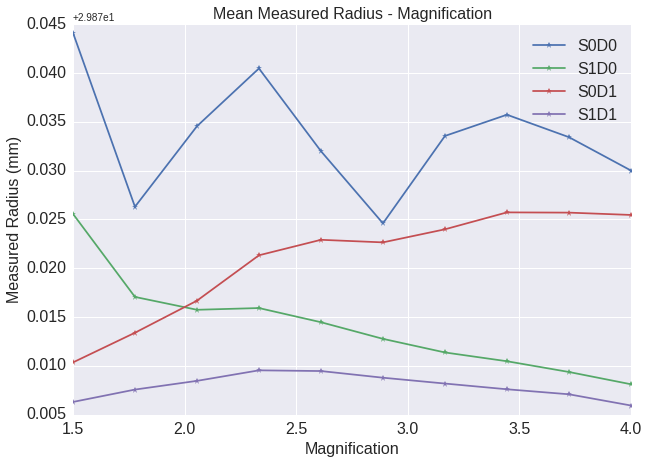
\includegraphics[width=\textwidth]{figures/output_10_0.png}
    \caption{Showing the average radius at each magnification.}
    \label{avgmeasuredradius}
\end{figure}

We can also look at the relative error of the measurements since we are in the position of knowing the true value - this can be seen in figure \ref{relerrormeasuredradius}. The $S0D0$ treatment shows the lowest relative errors of all treatments, there appears to be an increase in the error as magnification increases however the data is rather noisy. Treatments $S1D0$ and $S0D1$ show opposing, possibly linear, trends. Measurements taken with a non-ideal detector seem to get more accurate as magnification increases whereas the measurements taken with a non-ideal source show a decrease in the accuracy with an increase in magnification. When the measurements are taken with both non-ideal source and detector the relative errors are the largest of all treatments. There appears to be a non-linear, perhaps quadratic, relation between magnification and measurement error.

\begin{figure}[h!]
  \centering
    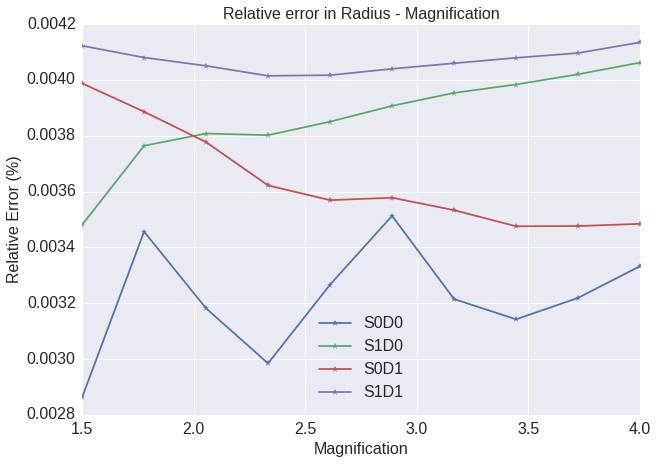
\includegraphics[width=\textwidth]{figures/output_8_0.png}
    \caption{Showing the relative error of the radius measurement at each magnification.}
        \label{relerrormeasuredradius}
\end{figure}

It should be noted that all the measured errors are at the sub-voxel level; the largest error seen is around $0.4\%$ which equates to an actual deviation from the true value of around $0.12$mm less then $2\%$ of the voxel width ($4.2$mm).

In figure \ref{stdmeasuredradius} we can see the variation (standard deviation) in the measurement in relation to magnification. This data is only available for $S1D0$, $S0D1$ and $S1D1$. This is because with an ideal source and detector the measurement is in effect deterministic. The projections do have very small additive noise applied but this is not enough to effect the reconstructions and hence the measurements in any meaningful way.

\begin{figure}[h!]
  \centering
    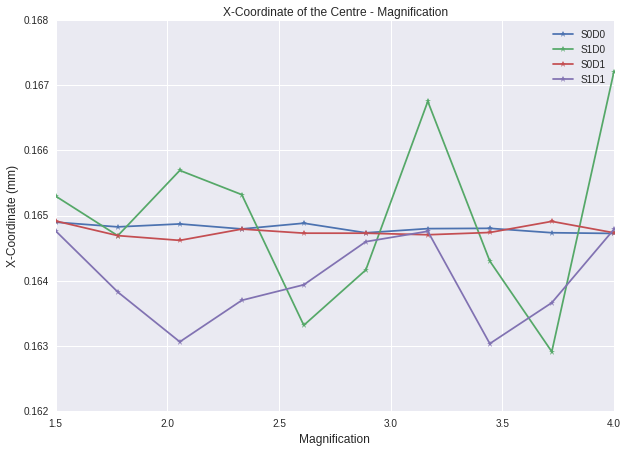
\includegraphics[width=\textwidth]{figures/output_14_0.png}
    \caption{Showing the variation of the radius measurement at each magnification.}
        \label{stdmeasuredradius}
\end{figure}

Any trend in the measurement variation is less clear to see. However if we ignore the data point at a magnification of $1.5$ for $S0D1$ it could be the case that the variation is decreasing with magnification for a non-ideal detector and vice-versa for a non-ideal source. In order to test this hypothesis a further twenty reconstructions were conducted at magnifications of $1.5$, $2.0556$ and $4.0$; the increase in sample size at these points should give a clearer picture of the underlying measurement variation. It would have been of great interest to conduct more reconstructions at all magnifications but this would have taken far too long - the new samples where chosen to cover low, medium and high magnifications in the hope that any trend became clearer. Figure \ref{stdmeasuredradiusxsamples} shows the measurement variation for the higher sampled magnifications. This seems to show that as magnification increases the measurement variability increase for the $S1D0$ treatment and decreases for the the $S0D1$ treatment. In order to further reinforce this conclusion two one tail T-tests where performed to see if the differences in the measurement variation was statistically significant. In the first test, which compares the measurement variance between $S1D0$ and  $S0D1$ at a magnification of $1.5$, the null and alternative hypothesis's are given by;

\[
H_0: \sigma_{S1D0,1.5} = \sigma_{S0D1,1.5}
\]
\[
H_1: \sigma_{S1D0,1.5} < \sigma_{S0D1,1.5}
\]

The test resulted in a p-value of $6.431e-06 < 0.01$, so the null hypothesis can be rejected at the 95\% level suggesting that there is significant evidence that $\sigma_{S1D0,1.5} < \sigma_{S0D1,1.5}$. For the second test we will compare the measurement variance between $S1D0$ and  $S0D1$ at a magnification of $4.0$. The null and alternative hypothesis's are given by;

\[
H_0: \sigma_{S1D0,4.0} = \sigma_{S0D1,4.0}
\]
\[
H_1: \sigma_{S1D0,4.0} > \sigma_{S0D1,4.0}
\]

The test resulted in a test statistic of a p-value of $2.347e-06 < 0.01$, so the null hypothesis can be rejected at the 95\% level suggesting that there is significant evidence that $\sigma_{S1D0,4.0} > \sigma_{S0D1,4.0}$. (NOTE: Need to report properly - give test statistic and critical value based on df = 29,29)

\begin{figure}[h!]
  \centering
    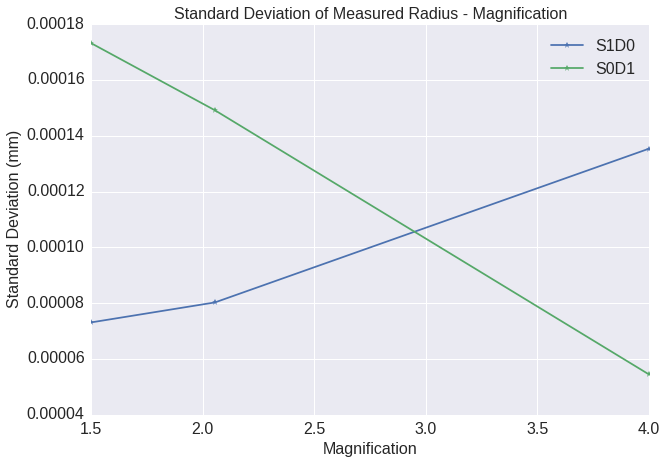
\includegraphics[width=\textwidth]{figures/output_34_0.png}
    \caption{Showing the variation of the radius measurement with a sample of 30 at each magnification.}
        \label{stdmeasuredradiusxsamples}
\end{figure}

\section{Image Resolution}
\section{Analytic MTF}
\chapter{Conclusion}




\end{document}
